\documentclass[10pt,a4paper]{amsart}
\usepackage[margin=19mm]{geometry}
\usepackage{amsmath,amssymb,mathtools}
\usepackage[scr=rsfs,cal=euler]{mathalfa}
\usepackage{xfrac}
\usepackage[unicode,hidelinks,bookmarks=false]{hyperref}
\newcommand{\ie}{i.e.\ }
\newcommand{\cf}{cf.\ }
\newcommand{\resp}{respectively\ }
\newcommand{\Subsection}{\subsection}
\providecommand{\nobreakdash}{\nobreak\hbox{-}}
\setlength{\emergencystretch}{2em}
\multlinegap0pt
\usepackage{tikz}
\usetikzlibrary{cd}
\usepackage{tikz}
\usepackage{amssymb}
\usepackage{enumerate}
\usepackage{mathtools}
\newtheorem{prop}{Proposition}
\newcommand{\ZZ}{\mathbb{Z}}
\DeclareMathOperator{\coker}{coker}
\DeclareMathOperator{\im}{im}
\newcommand{\rmH}{\mathrm{H}}
\title{On the Bogomolov-Positselski Conjecture}
\author{Julian Feuerpfeil}
\date{Source: arXiv:2503.09264v2 (CC BY 4.0)}
\begin{document}
\maketitle

\noindent\emph{Source and licence.} On the Bogomolov-Positselski Conjecture. Version arXiv:2503.09264v2 (CC BY 4.0), distributed by arXiv under the Creative Commons Attribution 4.0 International licence, http://creativecommons.org/licenses/by/4.0/, as recorded in the arXiv licence metadata for this exact version and shown on the abstract page https://arxiv.org/abs/2503.09264v2. Full licence notice: \texttt{licenses/arxiv-2503.09264-CC-BY-4.0.txt}.\par\smallskip

\noindent\textit{Editorial scope.} Counted unit: the article's prop prop:HomologicalAlgebra (source0.tex lines 422--437). The article's complete original proof of it is delivered with it (source0.tex lines 438--540, one \texttt{proof} environment of 103 lines). No mathematics is written, repaired or re-derived: the statement and the proof are the article's own lines, in the article's own notation, and no retained line is substituted or re-flowed.  Retained uncounted as the source-local context the proof needs: lines 293--299.  Nothing was omitted from any retained span, so the package carries no omission record.  No retained line contains a citation, so the wrapper carries no bibliography and no bibliography entry.  The retained lines contain the article's own diagram code, which the wrapper typesets with the standard tikz packages; no image file is delivered and the package declares no asset dependency.  Editorial formatting only, in addition: an AMS \texttt{amsart} preamble that restates the article's own declarations and macros used by the retained lines, namely the environments \texttt{prop} on separate counters, together with the standard packages those lines need.  The retained environments print in this document as Proposition 1 in order of appearance, whereas the article prints the same items with the numbering of its own full document.  The complete native source of the article as distributed in the arXiv e-print for this exact version is bundled unchanged as \texttt{sources/174630/source0.tex}.
\begin{prop}
\label{prop:CohomologyConcentrated}
    Let $A$ be a connected graded $k$-algebra and $M$ a graded $A$-module with $M_i=0$ for $i<m$ for some $m\in \ZZ$. Then for $j<i+m$ one has
    \begin{align*}
        \rmH_{ij}(A,M)=0\qquad\text{and}\qquad \rmH^{ij}(A,M)=0
    \end{align*}
\end{prop}

\begin{prop}
    \label{prop:HomologicalAlgebra}
    Let $A$ be a connected graded $k$-algebra and 
    \begin{equation*}
        0\to K\to M\overset{\varphi}{\to}A\overset{\pi}{\to}B\to 0
    \end{equation*}
     be an exact sequence of $A$-modules with degree preserving homomorphisms. Assume the following two conditions:
    \begin{enumerate}
        \item \label{ass:Mconcentrated} $M_i=0$ for $i< 1$ (thus $\pi$ is an isomorphism in degree $0$ and $1$);
        \item \label{ass:Kconcentrated} $K_i=0$ for $i<4$ (this implies with (\ref{ass:Mconcentrated}) that $\varphi$ is injective in degree $2$ and $3$);
    \end{enumerate}
    Then there is an exact sequence
    \begin{equation*}
            0\to H_{1,4}(A,M) \to H_{2,4}(A,B)\to K_4\to H_{0,4}(A,M)\to H_{1,4}(A,B)\to 0
    \end{equation*}
\end{prop}

\begin{proof}
    Consider the acyclic complex $C_*:=[0\leftarrow B\leftarrow A \leftarrow M\leftarrow K\leftarrow 0]$ (we choose $B$ to be in degree $0$, but it does not affect our arguments). Now, since the category of graded modules with degree preserving homomorphisms has enough projectives, there exist (projective) Cartan-Eilenberg resolutions, there is a homological spectral sequence $D^1_{s,t}:=H_{t,4}(A,C_s)\Rightarrow 0$. Since $D^1$ is concentrated in $4$ columns, we conclude $D^4_{s,t}=0$ for all $s$ and $t$. We denote the differentials by $\partial^r_{s,t}$.

    As $A$ is a free $A$ module, we have ${D}{^1_{1,t}}=0$ for all $t$ and by assumption (\ref{ass:Kconcentrated}) $\rmH_{0,4}(A,K)\cong K_4$. A variant of Proposition~\ref{prop:CohomologyConcentrated} implies $H_{i,4}(A,K)=0$ for $i\geq 1$ and similarly $H_{i,4}(A,M)=0$ for $i\geq 3$ (by assumption (\ref{ass:Mconcentrated})). Additionally $H_0(A,B)=B\otimes_Ak=k$, which is concentrated in degree $0$. Thus, we see that the first page of the spectral sequence can be described as depicted in Figure~\ref{fig:FirstPageOfD}.

    \begin{figure}[ht]
        \centering
        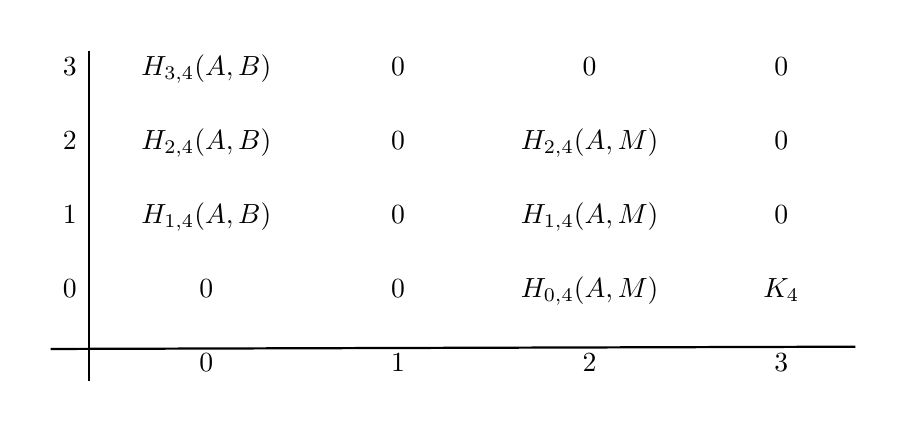
\begin{tikzpicture}
            \matrix (m) [matrix of math nodes,
                nodes={text width= 2cm,align=center, minimum height=5ex,outer sep=-5pt},
                column sep=.2cm,row sep=1ex,
                column 1/.style={nodes={text width=.6cm}}
                ]{
                    %Insert the entries of the spectral sequence here
                   % 4     &   0  &   0   &   0   &  0   \\
                    3     &   H_{3,4}(A,B)    &   0    &    0    &  0  \\
                    2     &   H_{2,4}(A,B)    &   0  &   H_{2,4}(A,M)     &  0  \\
                    1     &   H_{1,4}(A,B)    &   0   &    H_{1,4}(A,M)    &   0 \\
                    0     &   0   &    0    &   H_{0,4}(A,M)     &  K_4 \\
                \quad\strut &   0  &  1  &  2  & 3   \\};
            
                %Insert the name of the spectral sequence
                %\draw (m.west) node[left=.5cm] {${D}{^1_{*,*}}$};
                
                \draw[thick] (m-1-1.north east) -- (m-\the\pgfmatrixcurrentrow-1.south east) ;
                \draw[thick] (m-\the\pgfmatrixcurrentrow-1.north west) -- (m-\the\pgfmatrixcurrentrow-\the\pgfmatrixcurrentcolumn.north east) ;
                %\draw[thick,->] (m-3-3.east) -- (m-4-5.west);
                %\draw[->] (m-4-5.west) -- node[above]{$\partial_{3,0}^1(4)$} (m-4-4.east);
        \end{tikzpicture}
        \caption{First page of the spectral sequence $D^1_{*,*}$}
        \label{fig:FirstPageOfD}
    \end{figure}
    
The only non-zero differential on the first page is is ${\partial}{^1_{3,0}}:K_4\to \rmH_{0,4}(A,M)$. The resulting second page is shown in Figure~\ref{fig:SecondPageOfD}.


    \begin{figure}[ht]
        \centering
        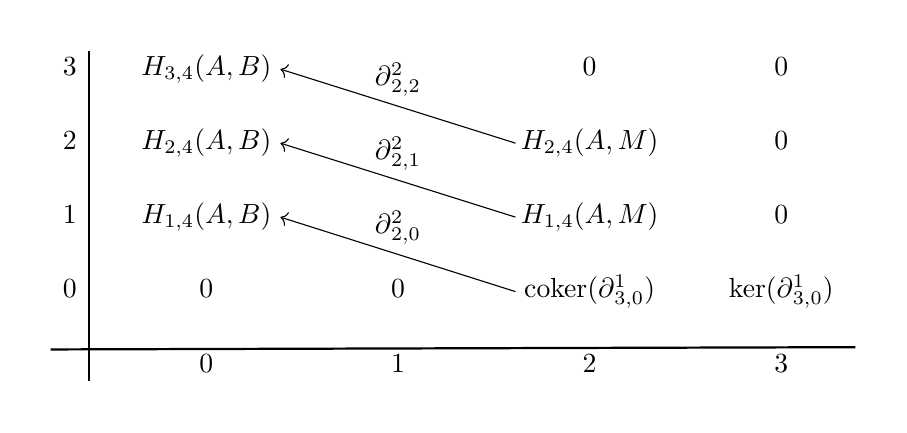
\begin{tikzpicture}
            \matrix (m) [matrix of math nodes,
                nodes={text width= 2cm,align=center, minimum height=5ex,outer sep=-5pt},
                column sep=.2cm,row sep=1ex,
                column 1/.style={nodes={text width=.6cm}}
                ]{
                    %Insert the entries of the spectral sequence here
                   % 4     &   0  &   0   &   0   &  0   \\
                    3     &   H_{3,4}(A,B)    &       &    0    &  0  \\
                    2     &   H_{2,4}(A,B)    &     &   H_{2,4}(A,M)     &  0  \\
                    1     &   H_{1,4}(A,B)    &      &    H_{1,4}(A,M)    &   0 \\
                    0     &   0   &    0    &   \coker({\partial}{^1_{3,0}})    &  \ker({\partial}{^1_{3,0}})  \\
                \quad\strut &   0  &  1  &  2  & 3   \\};
            
                %Insert the name of the spectral sequence
                %\draw (m.west) node[left=.5cm] {${D}{^2_{*,*}}$};
                
                \draw[thick] (m-1-1.north east) -- (m-\the\pgfmatrixcurrentrow-1.south east) ;
                \draw[thick] (m-\the\pgfmatrixcurrentrow-1.north west) -- (m-\the\pgfmatrixcurrentrow-\the\pgfmatrixcurrentcolumn.north east) ;
                \draw[->] (m-4-4.west) -- node[above] {${\partial}{^2_{2,0}}$} (m-3-2.east);
                \draw[->] (m-3-4.west) -- node[above] {${\partial}{^2_{2,1}}$} (m-2-2.east);
                \draw[->] (m-2-4.west) -- node[above] {${\partial}{^2_{2,2}}$} (m-1-2.east);
        \end{tikzpicture}
        \caption{Second page of the spectral sequence $D^2_{*,*}$}
        \label{fig:SecondPageOfD}
    \end{figure}

We conclude that all the maps ${\partial}{^2_{2,t}}$ are injective as $\ker ({\partial}{^2_{2,t}})={D}{^3_{2,t}}={D}{^\infty_{2,t}}$. Moreover, ${\partial}{^2_{2,0}}$ and ${\partial}{^2_{2,2}}$ have to be isomorphisms. Thus, the third page has only two non-zero entries is described in Figure~\ref{fig:ThirdPageOfD}.

    \begin{figure}[ht]
    \centering
        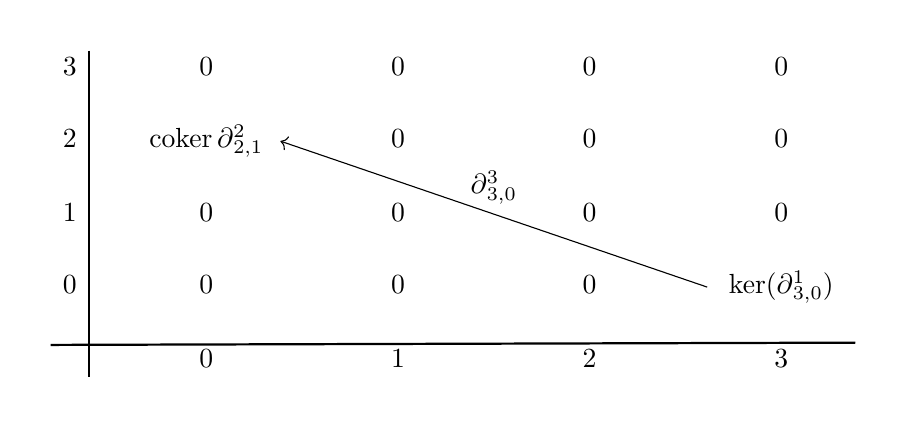
\begin{tikzpicture}
            \matrix (m) [matrix of math nodes,
                nodes={text width= 2cm,align=center, minimum height=5ex,outer sep=-5pt},
                column sep=.2cm,row sep=1ex,
                column 1/.style={nodes={text width=.6cm}}
                ]{
                    %Insert the entries of the spectral sequence here
                   % 4     &   0  &   0   &   0   &  0   \\
                    3     &   0    &   0    &    0    &  0  \\
                    2     &   \coker{\partial}{^2_{2,1}}   &   0  &   0     &  0  \\
                    1     &   0    &   0   &    0    &   0 \\
                    0     &   0   &    0    &   0    &  \ker({\partial}{^1_{3,0}})  \\
                \quad\strut &   0  &  1  &  2  & 3   \\
                };
            
            %Insert the name of the spectral sequence
            %\draw (m.west) node[left=.5cm] {${D}{^3_{*,*}}$};
            
            \draw[thick] (m-1-1.north east) -- (m-\the\pgfmatrixcurrentrow-1.south east) ;
            \draw[thick] (m-\the\pgfmatrixcurrentrow-1.north west) -- (m-\the\pgfmatrixcurrentrow-\the\pgfmatrixcurrentcolumn.north east) ;
            \draw[->] (m-4-5.west) -- node[above] {${\partial}{^3_{3,0}}$} (m-2-2.east);
        \end{tikzpicture}
        \caption{Second page of the spectral sequence $D^2_{*,*}$}
        \label{fig:ThirdPageOfD}
    \end{figure}
Similarly to the discussion before, the differential ${\partial}{^3_{3,0}}$ has to be an isomorphism. Thus we arrive at two short exact sequences:
\begin{equation*}
    \begin{tikzcd}[row sep=small]
        0\arrow[r]&H_{1,4}(A,M)\arrow[r,"{{\partial}{^2_{2,1}}}"] &H_{2,4}(A,B)\arrow[r]&\ker({\partial}{^1_{3,0}})\arrow[r]&0\\
        0\arrow[r]&\im({\partial}{^1_{3,0}})\arrow[r] &H_{0,4}(A,M)\arrow[r]&H_{1,4}(A,B)\arrow[r]&0\\
    \end{tikzcd}
\end{equation*}
Splicing these sequences together yields the desired $5$-term exact sequence.
\end{proof}

\end{document}
